% Generated by pysimcount.pfseeds -- do not edit; regenerate instead.
% figure: A-measured-by-order -- Suzuki formulas of each order, r from: Measured $r$; median over seeds [1, 2, 3, 4, 5, 6, 7, 8, 9, 10], bars = min..max
% metric=cnot gatebase=cz merged
% seed 1: git_commit=01d3c275ceae2840002bd1aaea68f59b987c4975 git_dirty=False
% seed 2: git_commit=01d3c275ceae2840002bd1aaea68f59b987c4975 git_dirty=False
% seed 3: git_commit=01d3c275ceae2840002bd1aaea68f59b987c4975 git_dirty=False
% seed 4: git_commit=01d3c275ceae2840002bd1aaea68f59b987c4975 git_dirty=False
% seed 5: git_commit=01d3c275ceae2840002bd1aaea68f59b987c4975 git_dirty=False
% seed 6: git_commit=01d3c275ceae2840002bd1aaea68f59b987c4975 git_dirty=False
% seed 7: git_commit=01d3c275ceae2840002bd1aaea68f59b987c4975 git_dirty=False
% seed 8: git_commit=01d3c275ceae2840002bd1aaea68f59b987c4975 git_dirty=False
% seed 9: git_commit=01d3c275ceae2840002bd1aaea68f59b987c4975 git_dirty=False
% seed 10: git_commit=01d3c275ceae2840002bd1aaea68f59b987c4975 git_dirty=False
% derived: A-measured-by-order.tex with Lie-Trotter S1 removed by pysimcount.figdrop (Lie-Trotter S1 alone spans 45% of the original y-axis); removed legends: Lie-Trotter S1; source_sha256=f379d0f0034a989eebcc6d8017abdd4b2f4b6f57284dd3f5e3c13cd2722a269c
% derived: A-measured-by-order-no-lie-trotter.tex restyled by pysimcount.figuniform: extrapolated points (r from power-law fit) drawn in their series' measured style, style-key legend entries removed; extrapolated n = [13, 20]; source_sha256=3dbf41010036876abbb5d072a061459429e6cc5ed0be2fa09a68bf87e8d9f411
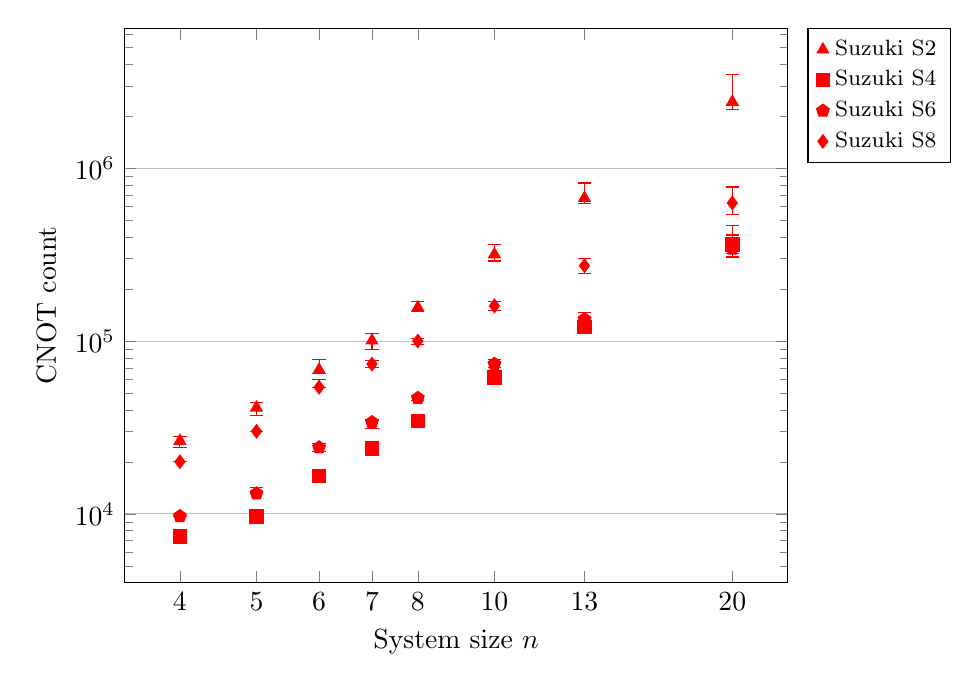
\begin{tikzpicture}
  \begin{loglogaxis}[
    width=10cm,
    xlabel={System size $n$},
    ylabel={CNOT count},
    xtick={4,5,6,7,8,10,13,20},
    xticklabels={4,5,6,7,8,10,13,20},
    ymajorgrids=true,
    legend pos=outer north east,
    legend cell align=left,
    legend style={font=\footnotesize},
  ]
    \addplot[only marks, red, mark=triangle*, mark size=2.4pt, mark options={solid, fill=red}, error bars/.cd, y dir=both, y explicit, error bar style={red}] coordinates {
      (4,26460) += (0,1500) -= (0,2300)
      (5,41200) += (0,2750) -= (0,4250)
      (6,68250) += (0,10230) -= (0,3150)
      (7,100765) += (0,9555) -= (0,10955)
      (8,156440) += (0,13400) -= (0,8360)
      (10,317650) += (0,43350) -= (0,26450)
    };
    \addlegendentry{Suzuki S2}
    \addplot[only marks, red, mark=triangle*, mark size=2.4pt, mark options={solid, fill=red}, forget plot, error bars/.cd, y dir=both, y explicit, error bar style={red}] coordinates {
      (13,673790) += (0,149630) -= (0,46410)
      (20,2428200) += (0,1074200) -= (0,230000)
    };
    \addplot[only marks, red, mark=square*, mark size=2.4pt, mark options={solid, fill=red}, error bars/.cd, y dir=both, y explicit, error bar style={red}] coordinates {
      (4,7392) += (0,168) -= (0,0)
      (5,9660) += (0,420) -= (0,210)
      (6,16632) += (0,1260) -= (0,756)
      (7,23961) += (0,2205) -= (0,1323)
      (8,34608) += (0,1344) -= (0,1344)
      (10,61530) += (0,5670) -= (0,1470)
    };
    \addlegendentry{Suzuki S4}
    \addplot[only marks, red, mark=square*, mark size=2.4pt, mark options={solid, fill=red}, forget plot, error bars/.cd, y dir=both, y explicit, error bar style={red}] coordinates {
      (13,120939) += (0,17199) -= (0,7917)
      (20,363720) += (0,102480) -= (0,42000)
    };
    \addplot[only marks, red, mark=pentagon*, mark size=2.4pt, mark options={solid, fill=red}, error bars/.cd, y dir=both, y explicit, error bar style={red}] coordinates {
      (4,9696) += (0,0) -= (0,0)
      (5,13130) += (0,1010) -= (0,0)
      (6,24240) += (0,1212) -= (0,1212)
      (7,33936) += (0,1414) -= (0,2828)
      (8,46864) += (0,1616) -= (0,1616)
      (10,73730) += (0,5050) -= (0,3030)
    };
    \addlegendentry{Suzuki S6}
    \addplot[only marks, red, mark=pentagon*, mark size=2.4pt, mark options={solid, fill=red}, forget plot, error bars/.cd, y dir=both, y explicit, error bar style={red}] coordinates {
      (13,133926) += (0,13130) -= (0,7878)
      (20,343400) += (0,68680) -= (0,36360)
    };
    \addplot[only marks, red, mark=diamond*, mark size=2.4pt, mark options={solid, fill=red}, error bars/.cd, y dir=both, y explicit, error bar style={red}] coordinates {
      (4,20040) += (0,0) -= (0,0)
      (5,30060) += (0,0) -= (0,0)
      (6,54108) += (0,6012) -= (0,0)
      (7,73647) += (0,3507) -= (0,3507)
      (8,100200) += (0,4008) -= (0,4008)
      (10,160320) += (0,10020) -= (0,10020)
    };
    \addlegendentry{Suzuki S8}
    \addplot[only marks, red, mark=diamond*, mark size=2.4pt, mark options={solid, fill=red}, forget plot, error bars/.cd, y dir=both, y explicit, error bar style={red}] coordinates {
      (13,273546) += (0,26052) -= (0,26052)
      (20,631260) += (0,150300) -= (0,90180)
    };
  \end{loglogaxis}
\end{tikzpicture}
